\section{Sistema propuesto}
Para este proyecto se planteó un sistema que implementa un lazo cerrado utilizando biofeedback. El sistema consiste en la adquisición de dos canales de sEMG, del brazo izquierdo, los cuales son procesados y sirven como entrada de un sistema de control que realiza la modulación de la amplitud de dos canales de estimulación eléctrica en el brazo derecho. Este sistema implementa un control contralateral para realizar un entrenamiento en espejo de las acciones de apertura y cierre de mano.

En la Figura \ref{Figura: SistProp} se muestra un esquema general del sistema desarrollado, en el cual se muestran en rojo los elementos sobre los cuales se trabajó en este proyecto.

\begin{figure}[htbp]
\centering
	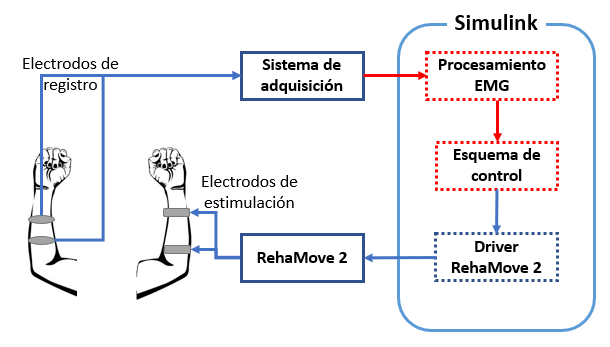
\includegraphics[scale=0.6]{SistemaPropuesto.png}
	\caption{Sistema propuesto para el proyecto. Líneas continuas representan entes de hardwares y líneas discontinuas representan entes de software. Elementos en rojo representan zonas de trabajo del proyecto.}
	\label{Figura: SistProp}
\end{figure}

\section{Adquisición de datos en Simulink}
Se utilizó el sistema Cyton Board (OpenBCI Inc., E.E. U.U. A.A.), el cual tiene una frecuencia de muestreo de 250 Hz, para realizar la adquisición de las señales de sEMG. Dicho sistema utiliza un chip ADS1299 (Texas Instruments) para realizar la conversión analógico-digital de las señales, el cual codifica los datos de cada muestra, utilizando complemento a 2, en un bus de datos esquematizado en la Figura \ref{Figura: BusOut}.

\begin{figure}[htbp]
\centering
	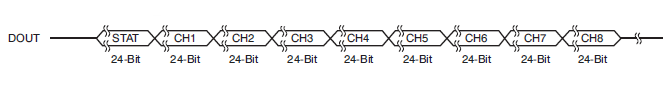
\includegraphics[scale=0.8]{Bus_Dat_Out_ADS.png}
	\caption{Estructura del bus de datos de salida del ADS1299}
	\label{Figura: BusOut}
\end{figure}

Para realizar la decodificación del bus de datos dentro de Simulink, se diseñó un subsistema encargado de la solicitud y decodificación de datos, para esto se utilizó el bloque \emph{Query Instrument} del \emph{Instrument Control Toolbox} para realizar la solicitud de datos, mientras que con bloques de la librería estándar de Simulink se realizó la decodificación de dichos datos.

El funcionamiento del subsistema responsable de la solicitud y decodificación de datos, esquematizado en la Figura \ref{Figura: DecoStream}, sigue los siguientes pasos:

\begin{enumerate}
	\item Realizar la adquisición de N muestras, lo cual generará un vector columna con dimensión (27*N,1).
	\item Aplicar un reshape a dicho vector para obtener una matriz con dimensión (27,N).
	\item Obtener la transpuesta de dicha matriz para obtener una matriz con dimension (N,27).
	\item Para cada canal, extraer de la matriz anterior las columnas asociadas a dicho canal de tal forma que se obtenga una submatriz con dimensión (N,3).
	\item Realizar una multiplicación matricial de dicha submatriz con un vector ponderador de tal forma que al final se obtenga un vector con dimensión (N,1) donde cada muestra n se encuentra en complemento a 2.
	\item Extraer del vector anterior las muestras en las que se encuentra codificado un número negativo (si el bit 23 de la muestra es 1 entonces se trata de un número negativo).
	\item Obtener el complemento a 1 de cada muestra del subvector obtenido, sumar 1 a cada muestra y por último multiplicar cada muestra por -1.
	\item Regresar los elementos del subvector al vector original.
\end{enumerate}

\begin{figure}[htbp]
\centering
	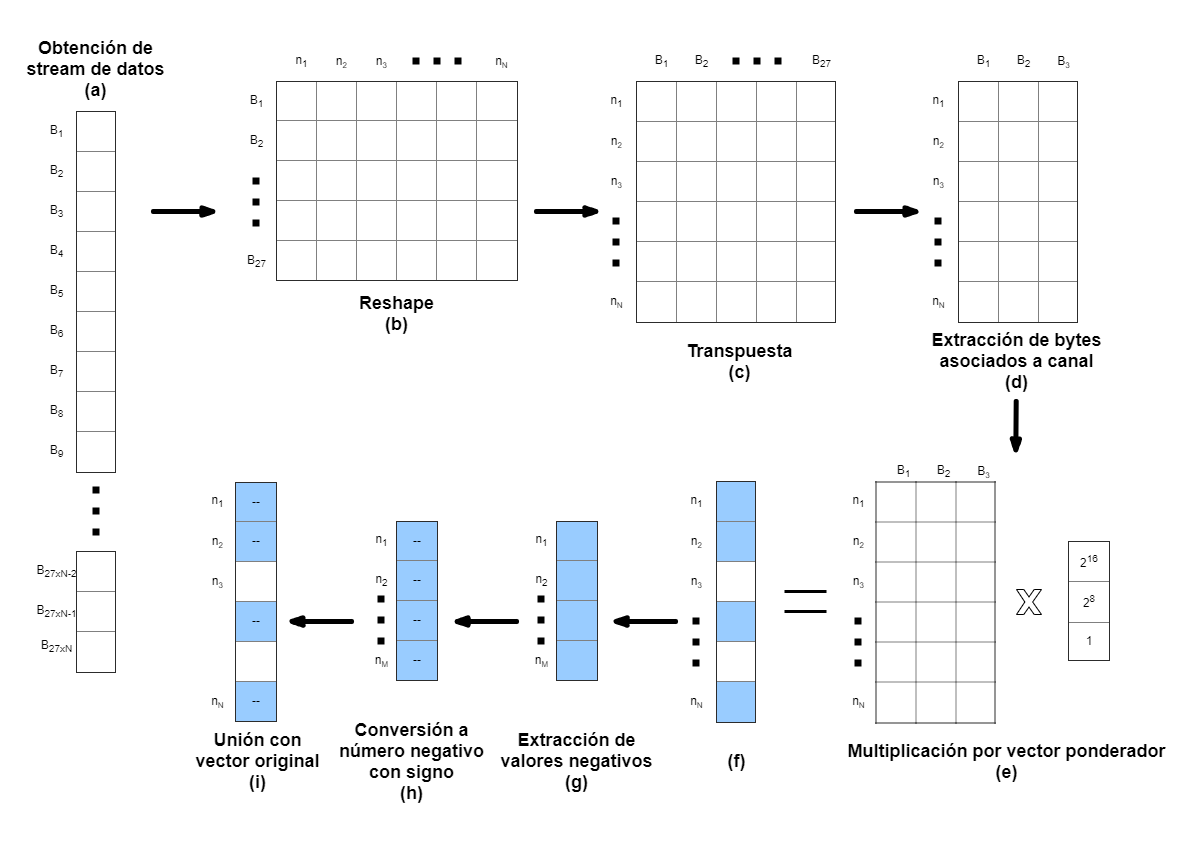
\includegraphics[scale=0.15]{DecoStream.png}
	\caption{Funcionamiento del subsistema decodificador del stream de datos}
	\label{Figura: DecoStream}
\end{figure}


La implementación final del subsistema diseñado en Simulink se observa en la Figura \ref{Figura: DecoSimuT}.

\begin{figure}[htbp]
	\centering
	\begin{subfigure}[htbp]{0.5\textwidth}
		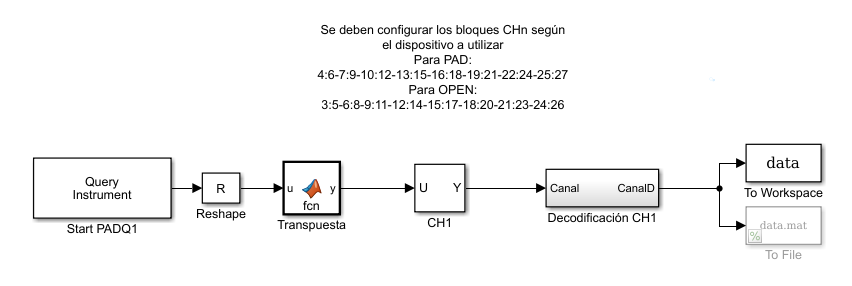
\includegraphics[width=\textwidth]{Read_Simu.png}
		\caption{Vista general del sistema diseñado para realizar adquisición y decodificación del stream de datos.}
		\label{Figura: readSimu}
	\end{subfigure}
	\begin{subfigure}[htbp]{0.5\textwidth}
		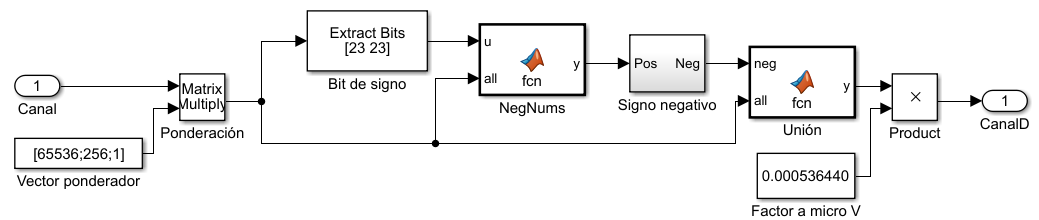
\includegraphics[width=\textwidth]{Deco_Simu.png}
		\caption{Vista interna del subsistema encargado de la decodificación del stream de datos.}
		\label{Figura: decoSimu}
	\end{subfigure}
	\caption{Sistema decodificador de stream de datos implementado en Simulink}
	\label{Figura: DecoSimuT}
\end{figure}

\section{Evaluación de bloque de adquisición y decodificación}
Para obtener una valoración sobre el funcionamiento del bloque diseñado dentro de Simulink para la adquisición y decodificación se generaron señales sintéticas dentro de MATLAB para que sirvieran como patrón de evaluación. Dichas señales consistieron en un banco de 5 senoidales a diferentes frecuencias (1 Hz, 5 Hz, 10 Hz, 20 Hz y 50 Hz (Figura \ref{Figura: SenPur})), dos senoidales de 50 Hz moduladas en amplitud con una exponencial decreciente (Figura \ref{Figura: ExpAte}) y una recta con pendiente negativa (Figura \ref{Figura: LinAte}), y una senoidal de 50 Hz modulada de tal forma que simule un contracción muscular que sube, se mantiene por un tiempo y baja (Figura \ref{Figura: Contra}). La duración de estas señales es de 5 segundos cada una, exeptuando la última que tiene una duración de 15 segundos, y todas se diseñaron con una frecuencia de muestreo de 250 Hz.

%Figura de senoidales MATLAB
\begin{figure}[htbp]
	\centering
	\begin{subfigure}[htbp]{0.4\textwidth}
		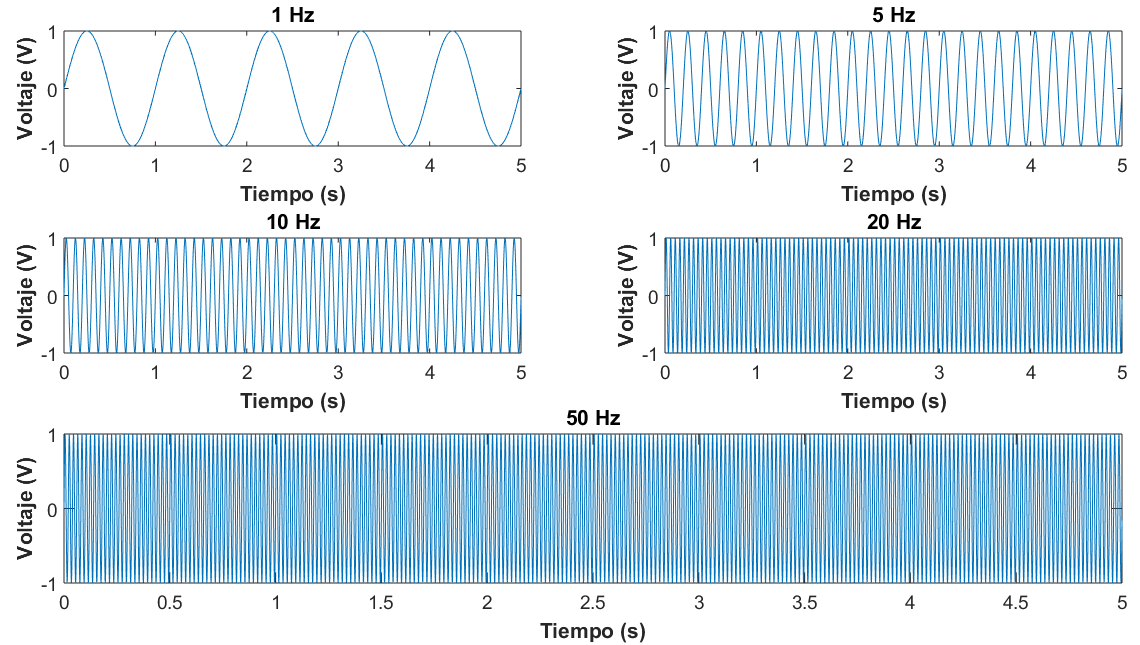
\includegraphics[width=\textwidth]{Sen_Pur.png}
		\caption{Senoidales puras a diferentes frecuencias}
		\label{Figura: SenPur}
	\end{subfigure}
	\hfill
	\begin{subfigure}[htbp]{0.4\textwidth}
		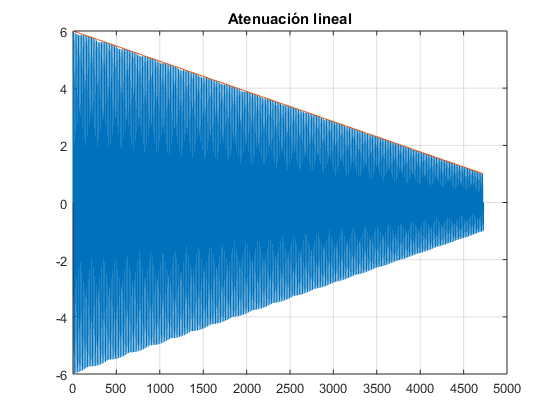
\includegraphics[width=\textwidth]{Lin_Ate.png}
		\caption{Senoidal de 50 Hz con atenuación lineal}
		\label{Figura: LinAte}
	\end{subfigure}
	\hfill
	\begin{subfigure}[htbp]{0.4\textwidth}
		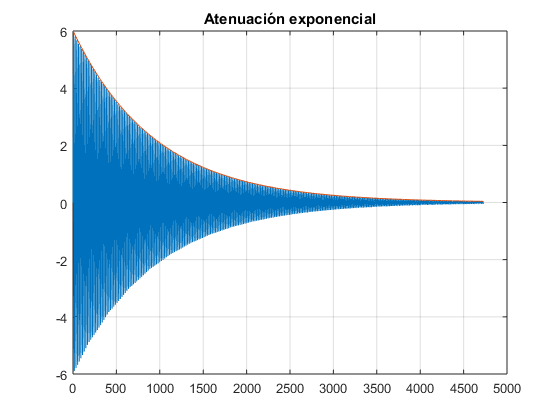
\includegraphics[width=\textwidth]{Exp_Ate.png}
		\caption{Senoidal de 50 Hz con atenuación exponencial}
		\label{Figura: ExpAte}
	\end{subfigure}
	\hfill
	\begin{subfigure}[htbp]{0.4\textwidth}
		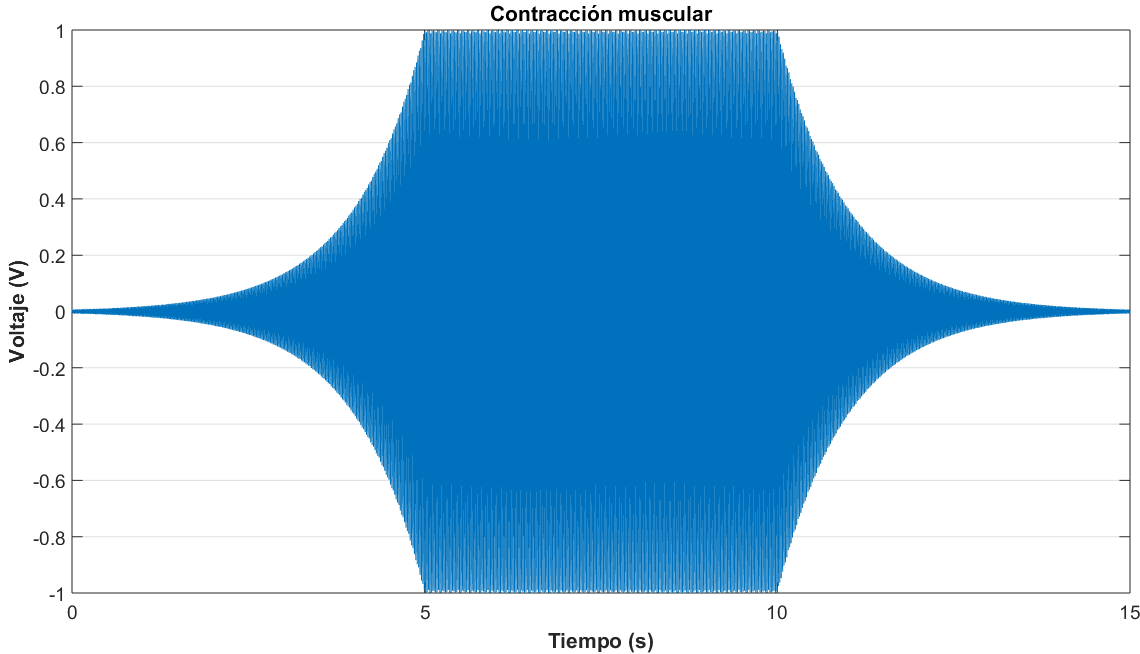
\includegraphics[width=\textwidth]{Contra.png}
		\caption{Senoidal de 50 Hz simulando una contracción muscular}
		\label{Figura: Contra}
	\end{subfigure}	
	\caption{Señales creadas para la evaluación del protocolo de comunicación}
	\label{Figura: SenalesEva}
\end{figure}

El proceso de evaluación se realizó de la siguiente manera:
\begin{enumerate}
	\item Utilizando un jack de audio de 3.5 mm, se conectó una punta a la salida de audio de la computadora, mientras que la otra punta se conectó al canal 1 del sistema de adquisición.
%	\item El canal 1 del prototipo de adquisición se configuró con una ganancia de 1 y se hablilitó el BIAS para dicho canal. La frecuencia de muestreo del prototipo se configuró a 1 kHz.
	\item Se inició la solicitud de datos utilizando el subsistema decodificador implementado en Simulink y se inició el contento de un cronómetro.
	\item Tras haber transcurridos 2 segundo en el cronómetro, se procedió a la reproducción de la señal tratándola como una señal de audio en MATLAB.
	\item Al marcar el cronómetro 10 segundos (20 segundos para la señal de larga duración), se detuvo la adquisición en el sistema de Simulink.
	\item Se calculó la métrica de correlación entre ambas señales como indicador de la calidad de la transferencia de datos.
\end{enumerate}

Estos pasos se repitieron tres veces para cada señal, esto para tener una mayor cantidad de datos con los cuales obtener una métrica de correlación promedio.

\section{Protocolo para registro de sEMG}
Para garantizar una repetibilidad en los registros de sEMG se implementó un protocolo para realizar la adquisición de dicha señal. Dicho protocolo tiene las caracteristicas mostradas a continuación:

\begin{itemize}
	\item Frecuencia de muestro de sistema de adquisición: 250 Hz.
	\item Canales 1 y 2 para realizar adquisición.
	\item Electrodos: Covidien H124SG
	\item Canal 1: Digitorum flexor
	\begin{itemize}
		\item Medir antebrazo de lado ventral de codo a muñeca.
		\item Palpar músculo al 25\% de la medida obtenida.
		\item Colocar dos electrodos separados 2 cm (Figura \ref{Figura: E_Cie}).
	\end{itemize}
	\item Canal 2: Digitorum extensor
	\begin{itemize}
		\item Medir antebrazo de lado dorsal de codo a muñeca.
		\item Palpar músculo al 50\% de la medida obtenida.
		\item Colocar dos electrodos separados 2 cm (Figura \ref{Figura: E_Ape}).
	\end{itemize}
	\item Referencia: Colocar electrodo en codo.
\end{itemize}

\begin{figure}[htbp]
	\centering
	\begin{subfigure}[htbp]{0.3\textwidth}
		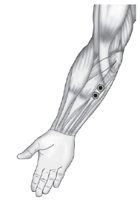
\includegraphics[width=\textwidth]{E_Cie.png}
		\caption{Ubicación de electrodos para digitorum flexor.}
		\label{Figura: E_Cie}
	\end{subfigure}
	\hfill
	\begin{subfigure}[htbp]{0.3\textwidth}
		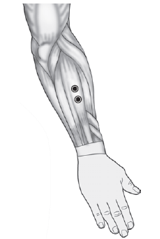
\includegraphics[width=\textwidth]{E_Ape.png}
		\caption{Ubicación de electrodos para digitorum extensor.}
		\label{Figura: E_Ape}
	\end{subfigure}
	\caption{Posicionamiento de electrodos para realizar registros de sEMG. Recuperado de \cite{Cavalcanti-Garcia2009}.}
	\label{Figura: E_sEMG}
\end{figure}

\section{Procesamiento de sEMG}

Se diseñaron tres filtros Butterworth para realizar el procesamiento de sEMG: un filtro pasa altas con frecuencia de corte de 15 Hz,para eliminar las variaciones en la línea base del registro; un filtro pasa bajas con frecuencia de corte de 100 Hz, para eliminar armónicos de 60 Hz y demás interferencias de alta frecuencia; y un filtro rechaza banda centrado en 60 Hz, para reducir la interferencia de la línea. Las gráficas de respuesta en frecuencia de estos filtros se muestran en las Figuras \ref{Figura: FiltroPA} a \ref{Figura: FiltroRB}.

\begin{figure}[htbp]
	\centering
	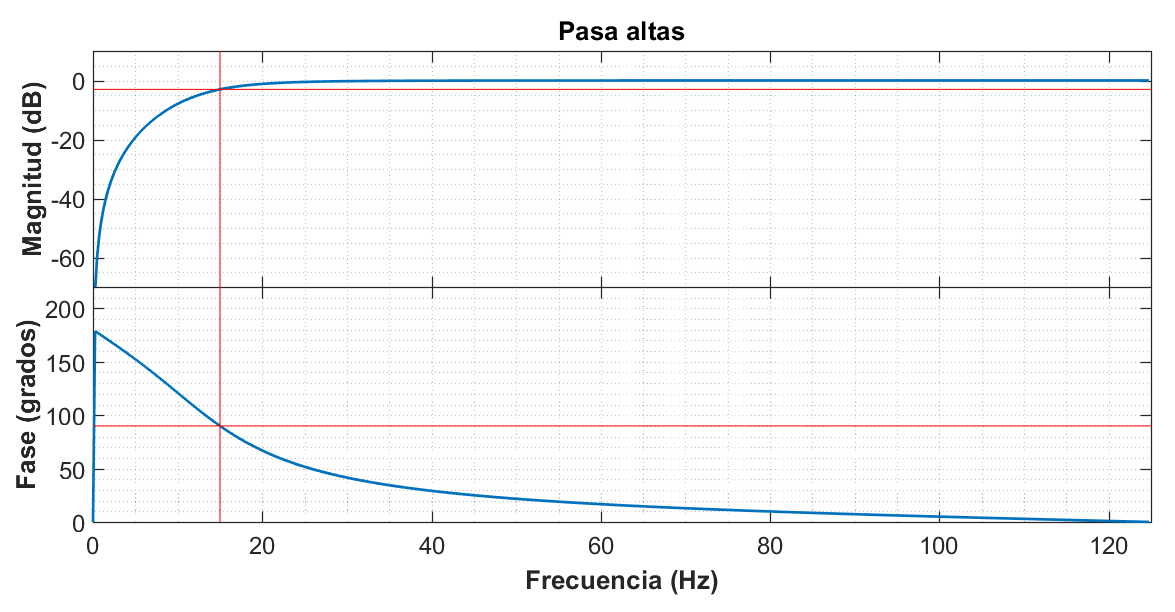
\includegraphics[width=0.7\textwidth]{FiltroPA15Hz_PADQ.png}
	\caption{Filtro pasa altas para conseguir línea base estable.}
	\label{Figura: FiltroPA}
	
	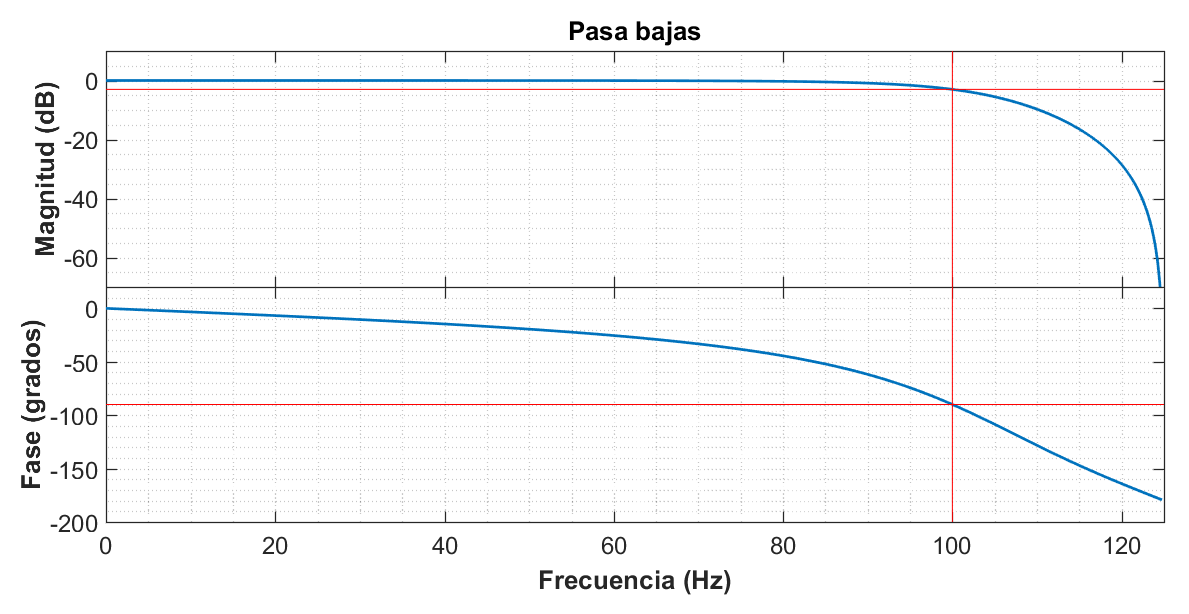
\includegraphics[width=0.7\textwidth]{FiltroPB100Hz_PADQ.png}
	\caption{Filtro pasa bajas para eliminar interferencias de alta frecuencia y armónicos de 60 Hz.} 
	\label{Figura: FiltroPB}
	
	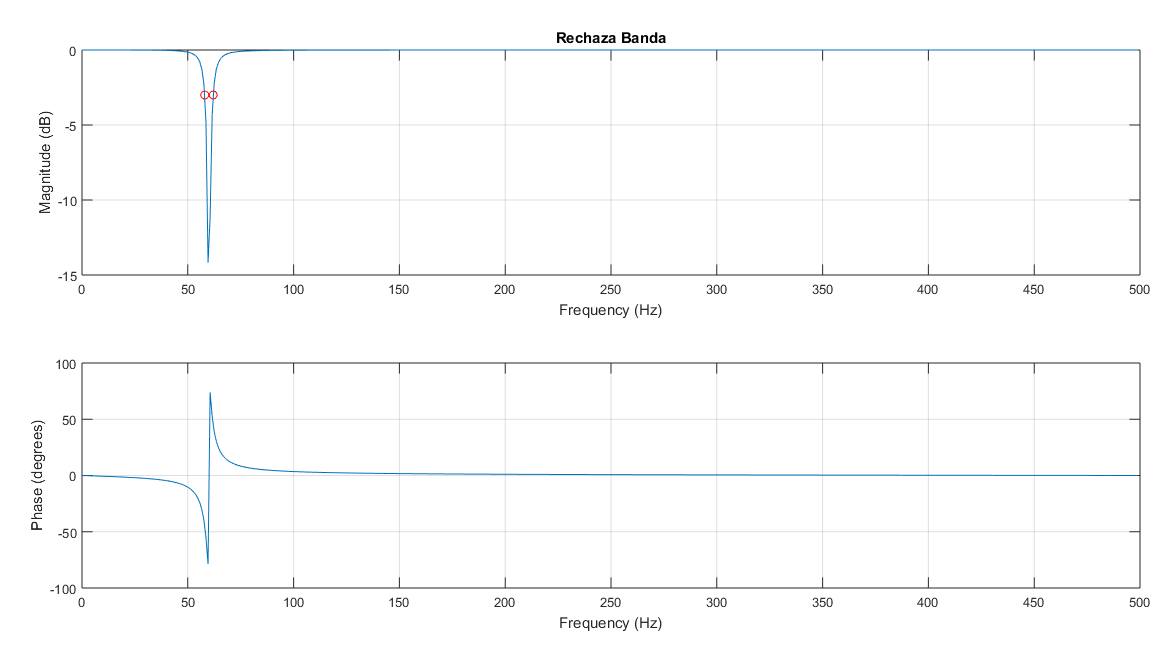
\includegraphics[width=0.7\textwidth]{FiltroRB_58_62_PADQ.png}
	\caption{Filtro rechaza banda para reducir interferencia de 60 Hz.}
	\label{Figura: FiltroRB}
\end{figure}

Se implementó dentro de Simulink un bloque responsable de obtener el valor RMS de ventanas de registro de 100 ms de sEMG para utilizar dicho descriptor de amplitud como señal de control. Adicionalmente se implementó un filtro de de mediana de 10 muestras (Ecuación \ref{Mediana}), el cual tiene como propósito conseguir una señal de RMS suavizada

\begin{equation}
	y[n] = mediana(x[n]:x[n-N])
	\label{Mediana}
\end{equation}

\newpage
\section{Esquema de control}
Se diseñó un sistema basado en una combinación de máquina de estados finitos con un control lineal. El sistema requiere de un proceso de calibración previa donde se obtienen 8 umbrales tras la repetición de 4 movimientos, dos umbrales corresponden a los valores RMS promedio de los dos canales de adquisición a lo largo de la tarea \emph{cierre de mano ligero}, otros dos corresponden a los valores RMS promedio de la tarea \emph{cierre de mano completo}, mientras que los 4 restantes corresponden a los valores RMS promedio de las tareas \emph{apertura de mano ligera} y \emph{apertura de mano completa}. {\color{red}AGREGAR FOTO DE POSTURAS DE MANOS}. Además, tras la calibración se obtiene también un factor denominado \emph{detector de movimiento}, el cual se obtiene tras calcular la diferencia promedio entre los canales de adquisición a lo largo de la tarea de apertura de mano. Adicionalmente se realiza una calibración de la estimulación eléctrica, la cual utiliza el sistema de colocación de electrodos de estimulación descrito en [{\color {red}ANA}], donde se obtiene los valores en amplitud de los umbrales motores y funcionales de las tareas de apertura y cierre de mano.

El detector de movimiento se utiliza para realizar el control por máquina de estados finitos ({\color{red}Figura NUM}), la cual consisten en determinar si la diferencia de amplitudes entre canales ha pasado el valor del detector de movimiento, si es así, el control prosigue con la tarea de apertura de mano, en caso contrario, el control procede a la tarea de cierre de mano.

Dentro del control de cada tarea, se utilizan los umbrales de las tareas ligeras para realizar la activación del control lineal, el cual modula la amplitud de la corriente eléctrica, del canal asociado al movimiento detectado, utilizando la recta descrita por la Ecuación \ref{Mapeo}, donde $A$ representa la amplitud que inyectará el estimulador eléctrico, $A_{max}$ es el umbral funcional de estimulación eléctica, $A_{min}$ es el umbral motor de estimulación eléctica, $D$ representa el valor RMS actual, mientras que $D_{max}$ y $D_{min}$ representan los umbrales RMS de la tarea completa y ligera del canal asociado al movimiento detectado (canal 1 para cierre de mano y canal 2 para apertura de mano). Adicionalmente se aplica la función máximo entero a la recta debido a que el dispositivo de estimulación eléctrica sólo admite valores enteros, y también se aplica un criterio de saturación de corriente eléctrica para evitar que tras una contracción muscular muy fuerte se genere un valor de amplitud de corriente eléctrica dañino para el sujeto.

\begin{equation}
	A = \frac{A_{max} - A_{min}}{D_{max} - D_{min}}(D - D_{min}) + A_{min}
	\label{Mapeo}
\end{equation}
